\chapter{\inverseMatTitle}
\label{inverse_matrix}


\begin{definition}
A square matrix $M$ is \emph{invertible} (or \emph{nonsingular})\index{Invertible}\index{Nonsingular} if there exists a matrix $M^{-1}$ such that
\[
M^{-1}M=I=M^{-1}M.
\]
\end{definition}

%\begin{figure}
%\begin{center}
%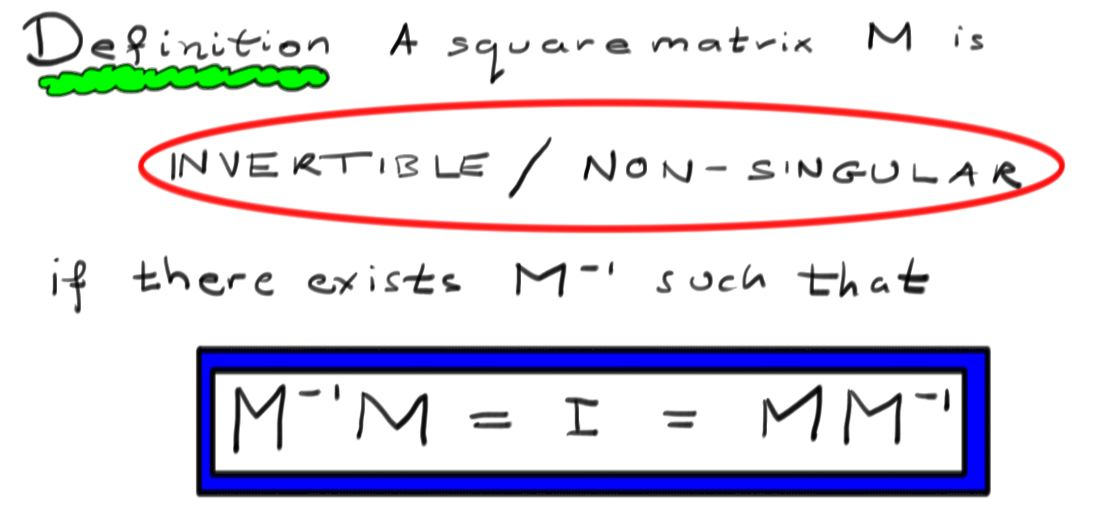
\includegraphics[scale=.27]{\inverseMatPath/defn_inverse_matrix.jpg}
%\end{center}
%\end{figure}


\begin{remark}[Inverse of a $2\times 2$ Matrix] Let $M$ and $N$ be the matrices:
\[
M=\begin{pmatrix}
a & b \\
c & d \\
\end{pmatrix},\qquad N=\begin{pmatrix}
d & -b \\
-c & a \\
\end{pmatrix}
\]
Multiplying these matrices gives:
\[
MN=\begin{pmatrix}
ad-bc & 0 \\
0 & ad-bc \\
\end{pmatrix}=(ad-bc)I
\]

Then $M^{-1}=\frac{1}{ad-bc}\begin{pmatrix}
d & -b \\
-c & a \\
\end{pmatrix}$, so long as $ad-bc\neq 0$.    
\end{remark}

\begin{figure}
\begin{center}
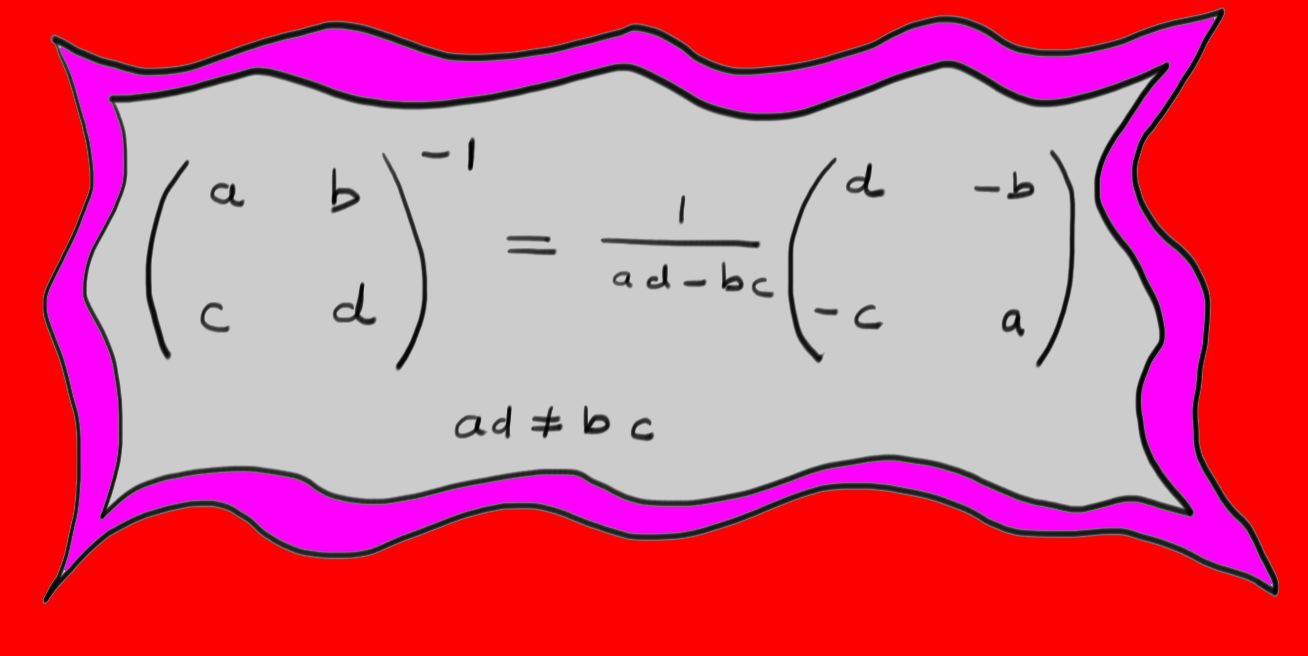
\includegraphics[scale=.24]{\inverseMatPath/2x2_inverse.jpg}
\end{center}
\caption{The formula for the inverse of a 2$\times$2 matrix is worth memorizing!}
\end{figure}



\section{Three Properties of the Inverse}

\begin{enumerate}
\item If $A$ is a square matrix and $B$ is the inverse of $A$, then $A$ is the inverse of $B$, since $AB=I=BA$.  Then we have the identity:
\[
(A^{-1})^{-1}=A
\]

\item Notice that $B^{-1}A^{-1}AB=B^{-1}IB=I=ABB^{-1}A^{-1}$.
Then:
\[
(AB)^{-1}=B^{-1}A^{-1}
\]
Then much like the transpose, taking the inverse of a product \emph{reverses} the order of the product.


\begin{center}
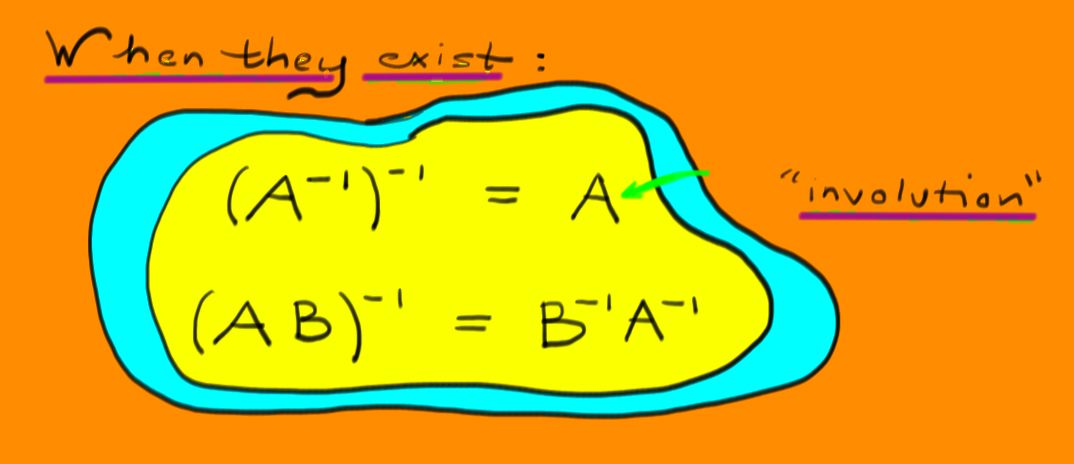
\includegraphics[scale=.26]{\inverseMatPath/inverse_inverse.jpg}
\end{center}

\item Finally, recall that $(AB)^T=B^TA^T$.  Since $I^T=I$, then $(A^{-1}A)^T=A^T(A^{-1})^T=I$.  Similarly, $(AA^{-1})^T=(A^{-1})^TA^T=I$.  Then:
\[
(A^{-1})^T=(A^T)^{-1}
\]
%As such, we could even write $A^{-T}$ for the inverse of the transpose of $A$ (or equivalently the transpose of the inverse).
\begin{center}
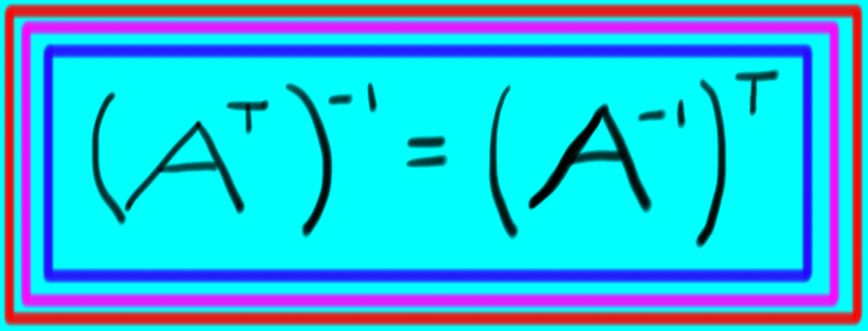
\includegraphics[scale=.20]{\inverseMatPath/transpose_inverse.jpg}
\end{center}
\end{enumerate}

\videoscriptlink{inverse_matrix_2by2_example.mp4}{Example}{scripts_inverse_matrix_2by2_example}




\section{Finding Inverses}

Suppose $M$ is a square matrix and $MX=V$ is a linear system with unique solution $X_0$.  Since there is a unique solution, $M^{-1}V$, then the reduced row echelon form of the linear system has an identity matrix on the left:
\[
\begin{amatrix}{1}
M & V
\end{amatrix}
\sim
\begin{amatrix}{1}
I & M^{-1}V
\end{amatrix}
\]
Solving the linear system $MX=V$ then tells us what $M^{-1}V$ is.  

To solve many linear systems with the same matrix at once, 
$$MX=V_1,~MX=V_2$$

we can consider augmented matrices with 
%a matrix on the right side instead of a column vector, 
many columns on the right 
 and then apply Gaussian row reduction to the left side of the matrix.  Once the identity matrix is on the left side of the augmented matrix, then the solution of each of the individual linear systems is on the right.
 \[
\left(\begin{array}{c|cc}
M & V_1&V_2
\end{array}\right)
\sim
\left(\begin{array}{c|cc}
I & M^{-1}V_1 & M^{-1}V_2
\end{array}\right)
\]


To compute $M^{-1}$, we would like $M^{-1}$, rather than $M^{-1}V$ to appear on the right side of our augmented matrix.
This is achieved by  solving the collection of systems $MX=e_k$, where $e_k$ is the column vector of zeroes with a $1$ in the $k$th entry.  
{\it I.e.,} the $n\times n$ identity matrix can be viewed as a bunch of column vectors $I_n=(e_1 \ e_2 \ \cdots e_n)$. So, putting the $e_k$'s together into an identity matrix, we get:
\[
\begin{amatrix}{1}
M & I
\end{amatrix}
\sim
\begin{amatrix}{1}
I & M^{-1}I
\end{amatrix}
=\begin{amatrix}{1}
I & M^{-1}
\end{amatrix}
\]


\begin{example}
Find $\begin{pmatrix}
-1 & 2 & -3 \\
2 & 1 & 0 \\
4 & -2 & 5 \\
\end{pmatrix}^{-1}
$.
Start by writing the augmented matrix, then apply row reduction to the left side.

\begin{eqnarray*}
\begin{pmat}{rrr|ccc}
-1 & 2 & -3 & 1 & 0 & 0 \\[1mm]
2  & 1 &  0 & 0 & 1 & 0 \\[1mm]
 4 & -2 & 5 & 0 & 0 & 1 \\[1mm]
\end{pmat} & \sim & \begin{pmat}{crr|ccc}
1  & -2&  3  & 1 & 0 & 0 \\[1mm]
0  & 5 &  -6 & 2 & 1 & 0 \\[1mm]
 0 & 6 & -7  & 4 & 0 & 1 \\[1mm]
\end{pmat} \\[2mm]
& \sim & \begin{pmat}{ccr|rrc}
1  & 0 &  \frac{3}{5}  & -\frac{1}{4} & \frac{2}{5} & 0 \\[1mm]
0  & 1 &  -\frac{6}{5} & \frac{2}{5} & \frac{1}{5}  & 0 \\[1mm]
 0 & 0 &  \frac{1}{5}  & \frac{4}{5} & -\frac{6}{5} & 1 \\[1mm]
\end{pmat} \\[2mm]
& \sim & \begin{pmat}{ccc|rrr}
1  & 0 &  0  & -5 & 4 & -3 \\[1mm]
0  & 1 &  0  & 10 & -7 & 6 \\[1mm]
 0 & 0 &  1  & 8 & -6 & 5 \\[1mm]
\end{pmat} \\
\end{eqnarray*}
At this point, we know $M^{-1}$ assuming we didn't goof up\index{Goofing up}.  However, row reduction is a lengthy and arithmetically involved process, so we should~\emph{check our answer,} by confirming that $MM^{-1}=I$ (or if you prefer $M^{-1}M=I$):
\[MM^{-1} = 
\begin{pmatrix}
-1 & 2 & -3 \\
2 & 1 & 0 \\
4 & -2 & 5 \\
\end{pmatrix}\begin{pmatrix}
-5 & 4 & -3 \\
10 & -7 & 6 \\
 8 & -6 & 5 \\
\end{pmatrix}
=\begin{pmatrix}
1 & 0 & 0 \\
0 & 1 & 0 \\
0 & 0 & 1 \\
\end{pmatrix}
\]  
The product of the two matrices is indeed the identity matrix, so we're done.
\end{example}

%\href{\webworkurl ReadingHomework10/1/}{Reading homework: problem 10.1}
\reading{10}{1}
\section{Linear Systems and Inverses}

If $M^{-1}$ exists and is known, then we can immediately solve linear systems associated to $M$.

\begin{example}
Consider the linear system:

\[
      \begin{linsys}{2}
            -x & +2y & -3z         &=& 1  \\[1mm]
            2x & +\ y\,   &             &=& 2 \\[1mm]
            4x & -2y & +5z         &=& 0  
      \end{linsys}
\]
The associated matrix equation is $MX=\colvec{1\\2\\0},$ where \(M\) is the same as in the previous section.  Then:

\[
\colvec{x\\y\\z}=\begin{pmatrix}
-1 & 2 & -3 \\
2 & 1 & 0 \\
4 & -2 & 5 \\
\end{pmatrix}^{-1}\colvec{1\\2\\0}
=\begin{pmatrix}
-5 & 4 & -3 \\
10 & -7 & 6 \\
 8 & -6 & 5 \\
\end{pmatrix}\colvec{1\\2\\0}
=\colvec{3\\-4\\-4}
\]
Then $\colvec{x\\y\\z}=\colvec{3\\-4\\-4}$.  
In summary, when $M^{-1}$ exists, then $$MX=V \Rightarrow X=M^{-1}V\, .$$
\end{example}



%\href{\webworkurl ReadingHomework10/2/}{Reading homework: problem 10.2}
\reading{10}{2}

\section{Homogeneous Systems}

\begin{theorem}
A square matrix $M$ is invertible if and only if the homogeneous system $$MX=0$$ has no non-zero solutions.
\end{theorem}

\begin{proof}
First, suppose that $M^{-1}$ exists.  Then $MX=0 \Rightarrow X=M^{-1}0=0$.  Thus, if $M$ is invertible, then $MX=0$ has no non-zero solutions.

On the other hand, $MX=0$ always has the solution $X=0$.  If no other solutions exist, then $M$ can be put into reduced row echelon form with every variable a pivot.  In this case, $M^{-1}$ can be computed using the process in the previous section.
\end{proof}

%\begin{figure}
\begin{center}
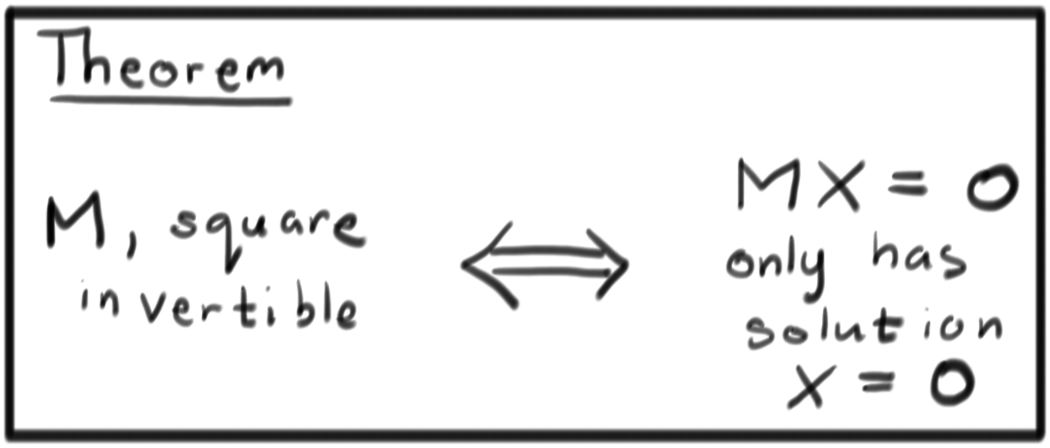
\includegraphics[scale=.26]{\inverseMatPath/inverse_theorem.jpg}
\end{center}
%\end{figure}

%A great test of your linear algebra knowledge is to make a list of conditions for a matrix to be singular.
%You will learn more of these as the course goes by, but can also skip straight to the list in Section~\ref{thelist}. 

\section{Bit Matrices}\index{Bit matrices}
In computer science, information is recorded using binary strings of data.  For example, the following string contains an English word:
\[
011011000110100101101110011001010110000101110010
\]
A \hypertarget{bits}{\emph{bit}} is the basic unit of information, keeping track of a single one or zero.  Computers can add and multiply individual bits very quickly.

Consider the set $\Z_2=\{0,1 \}$ with addition and multiplication given by the following tables:
\label{Z2}
\[
\begin{array}{c|cc}
+ & 0 & 1 \\ \hline
0 & 0 & 1 \\
1 & 1 & 0 \\
\end{array}
\qquad
\begin{array}{c|cc}
\cdot & 0 & 1 \\ \hline
0 & 0 & 0 \\
1 & 0 & 1 \\
\end{array}
\]
Notice that $-1=1$, since $1+1=0$.

It turns out that $\Z_2$ is almost as good as the real or complex numbers (they are all \hyperref[fields]{fields}), so we can apply all of the linear algebra we have learned thus far to matrices with $\Z_2$ entries.  A matrix with entries in $\Z_2$ is sometimes called a \emph{bit matrix}\footnote{Note that bits in a bit arithmetic shorthand do not ``add'' and ``multiply'' as elements in $\mathbb{Z}_2$ does since these operators corresponding to ``bitwise or'' and ``bitwise and'' respectively.}.

\begin{example}
$\begin{pmatrix}
1 & 0 & 1 \\
0 & 1 & 1 \\
1 & 1 & 1 \\
\end{pmatrix}$ is an invertible matrix over $\Z_2$:

\[\begin{pmatrix}
1 & 0 & 1 \\
0 & 1 & 1 \\
1 & 1 & 1 \\
\end{pmatrix}^{-1}=\begin{pmatrix}
0 & 1 & 1 \\
1 & 0 & 1 \\
1 & 1 & 1 \\
\end{pmatrix}
\]

This can be easily verified by multiplying:

\[\begin{pmatrix}
1 & 0 & 1 \\
0 & 1 & 1 \\
1 & 1 & 1 \\
\end{pmatrix}\begin{pmatrix}
0 & 1 & 1 \\
1 & 0 & 1 \\
1 & 1 & 1 \\
\end{pmatrix}=\begin{pmatrix}
1 & 0 & 0 \\
0 & 1 & 0 \\
0 & 0 & 1 \\
\end{pmatrix}
\]
\end{example}

\begin{remark}[Application: Cryptography]  
A very simple way to hide information is to use a substitution cipher, in which the alphabet is permuted and each letter in a message is systematically exchanged for another.  For example, the ROT-13 cypher just exchanges a letter with the letter thirteen places before or after it in the alphabet.  For example, HELLO becomes URYYB.  Applying the algorithm again decodes the message, turning URYYB back into HELLO.  Substitution ciphers are easy to break, but the basic idea can be extended to create cryptographic systems that are practically uncrackable.  For example, a \emph{one-time pad} is a system that uses a different substitution for each letter in the message.  So long as a particular set of substitutions is not used on more than one message, the one-time pad is unbreakable.

English characters are often stored in computers in the ASCII format.  In ASCII, a single character is represented by a string of eight bits, which we can consider as a vector in $\Z_2^8$ (which is like vectors in $\Re^8$, where the entries are zeros and ones).  One way to create a substitution cipher, then, is to choose an $8\times 8$ invertible bit matrix $M$, and multiply each letter of the message by $M$.  Then to decode the message, each string of eight characters would be multiplied by $M^{-1}$.  

To make the message a bit tougher to decode, one could consider pairs (or longer sequences) of letters as a single vector in $\Z_2^{16}$ (or a higher-dimensional space), and then use an appropriately-sized invertible matrix.

For more on cryptography, see ``The Code Book,'' by Simon Singh (1999, Doubleday).
\end{remark}

%{\it You should now be ready to attempt the \hyperref[sample1]{first sample midterm}.}
%\begin{center}
%\shabox{
%\begin{tabular}{c}
%\it \hyperref[sample1]{You are now ready to attempt the first sample midterm}. 
%\\
%\hyperref[sample1]{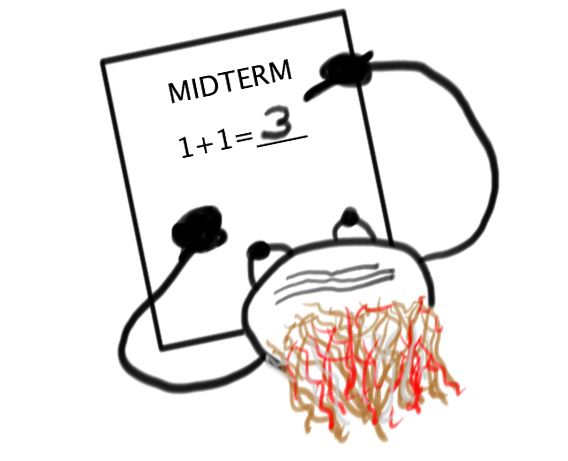
\includegraphics[scale=.15]{midterm.jpg}}
%\end{tabular}
%}
%\end{center}
%
%\section*{References}
%
%Hefferon: Chapter Three, Section IV.2
%\\
%Beezer: Chapter M, Section MISLE
%\\
%Wikipedia:
%\href{http://en.wikipedia.org/wiki/Invertible_matrix}{Invertible Matrix}
%
%
\section{Review Problems}



\begin{enumerate}

\item While performing  Gaussian elimination on these augmented matrices write the full system of equations describing the new rows in terms of the old rows above each equivalence symbol as in  \hyperlink{Keeping track of EROs with equations between rows}{Example}~\ref{Rsystem}. 
$$
\begin{amatrix}{2} 
2 & 2 & 10 \\
1 & 2 & 8 \\
\end{amatrix}
,~
\begin{amatrix}{3} 
1 & 1 & 0 & 5 \\
1 & 1 & \!\!-1& 11 \\
-1 & 1 & 1 & -5 \\ 
\end{amatrix}
$$

%%%%%%%%%%%%%%%%%%%

\item Solve the vector equation by applying ERO matrices to each side of the equation to perform elimination. Show each matrix explicitly as in \hyperlink{Undoing}{Example~\ref{slowly}}.

\begin{eqnarray*}
\begin{pmatrix}
3	&6 	&2 \\ %-3
5 	&9 	&4 \\ %1
2	&4	&2 \\ %0
\end{pmatrix} 
\begin{pmatrix}
 x \\ 
y \\
z 
\end{pmatrix} 
=
\begin{pmatrix}
-3 \\ 
1  \\
0  \\
\end{pmatrix} 
\end{eqnarray*}

%%%%%%%%%%%%%%%%%%%

\item Solve this vector equation by finding the inverse of the matrix through $(M|I)\sim (I|M^{-1})$ and then applying $M^{-1}$ to both sides of the equation. 
\begin{eqnarray*}
\begin{pmatrix}
2	&1 	&1 \\ %9
1 	&1 	&1 \\ %6
1	&1	&2 \\ %7
\end{pmatrix} 
\begin{pmatrix}
 x \\ 
y \\
z 
\end{pmatrix} 
=
\begin{pmatrix}
9 \\ 
6  \\
7  \\
\end{pmatrix} 
\end{eqnarray*}


%%%%%%%%%%%%%%%%%%%

\item Follow the method of  \hyperlink{elldeeeww}{Examples~\ref{factorize} and~\ref{factorizes}} to find the $LU$ and $LDU$ factorization of 
\begin{eqnarray*}
\begin{pmatrix}
3	&3 	&6 \\ %0 %2
3 	&5 	&2 \\ %1 %1
6	&2	&5 \\ %0 %1
\end{pmatrix} .
\end{eqnarray*}



%%%%%%%%%%%%%%%%%%%%

\item 
Multiple matrix equations with the same matrix can be solved simultaneously. 
\begin{enumerate}
\item Solve both systems by performing elimination on just one augmented matrix.
\begin{eqnarray*}
\begin{pmatrix}
2	&-1 	&-1 \\ %0 %2
-1 	&1 	&1 \\ %1 %1
1	&-1	&0 \\ %0 %1
\end{pmatrix} 
\begin{pmatrix}
 x \\ 
y \\
z 
\end{pmatrix} 
=
\begin{pmatrix}
0\\ 
1  \\
0  \\
\end{pmatrix} 
,~
\begin{pmatrix}
2	&-1 	&-1 \\ %0 %2
-1 	&1 	&1 \\ %1 %1
1	&-1	&0 \\ %0 %1
\end{pmatrix} 
\begin{pmatrix}
 a \\ 
b \\
c 
\end{pmatrix} 
=
\begin{pmatrix}
2\\ 
1  \\
1  \\
\end{pmatrix} 
\end{eqnarray*}
\item Give an interpretation of the columns of $M^{-1}$ in $(M|I)\sim (I|M^{-1})$ in terms of solutions to certain systems of linear equations.
\end{enumerate}

%%%%%%%%%%%%%%%%%%%%%%%%

\item How can you convince your fellow students to never make this mistake?
\begin{eqnarray*}
\begin{amatrix}{3} 
1 & 0 & 2 & 3 \\ 
0 & 1 & 2& 3 \\
2 & 0 & 1 & 4 \\
\end{amatrix} 
& 
\stackrel{R_1'=R_1+R_2}{
\stackrel{R_2'=R_1-R_2}{ 
\stackrel{\ R_3'= R_1+2R_2}{\sim}}}
&
\begin{amatrix}{3} 
1 & 1 & 4 & 6 \\
1 & \!\!-1 & 0& 0 \\
1 & 2 & 6 & 9 
\end{amatrix}
\end{eqnarray*}

\item Is $LU$ factorization of a matrix unique?  Justify your answer.


\item[$\infty$.] If you randomly create a matrix by picking numbers out of the blue, it will probably be difficult to perform elimination or factorization; fractions and large numbers will probably be involved. To invent simple problems it is better to start with a simple answer:
\begin{enumerate}
\item Start with any augmented matrix in RREF. Perform EROs to make most of the components non-zero. Write the result on a separate piece of paper and give it to your friend. Ask that friend to find RREF of the augmented matrix you gave them. Make sure they get the same augmented matrix you started with.  
\item Create  an upper triangular matrix $U$ and a lower triangular matrix~$L$ with only $1$s on the diagonal. Give the result to a friend to factor into $LU$ form. 
\item Do the same with an $LDU$ factorization. 
\end{enumerate}
\end{enumerate}

\phantomnewpage



\newpage


